\chapter{Политика}


\section{20 лет Владимира Путина: трансформация режима}

\textit{Политолог Кирилл Рогов открывает цикл статей о том, как изменилась страна за путинские годы}

\textit{Источник: \url{www.vedomosti.ru/opinion/articles/2019/08/07/808337-20-let-putina}}

\textit{Кирилл Рогов }

20 лет назад Владимир Путин внезапно появился на политическом олимпе в образе эффективного бюрократа с силовым бэкграундом, рыночно ориентированного государственника и прагматика, чуждого идеологических пафосов. Сегодня Путин выглядит сильным авторитарным лидером (типаж «стронгмен»), увлеченным геополитическим противостоянием с Западом и идейной борьбой с мировым либерализмом, решительно жертвующим ради этого прагматическими целями развития страны. И даже когда он заговаривает о модернизации, разговор довольно быстро сбивается на виды вооружений.

\textbf{Две эпохи}



Если бы Путин ушел в 2008 г., то остался бы в истории как один из самых успешных лидеров России. После 15 лет кризисов и пертурбаций в стране наступила относительная стабилизация на условиях «управляемой демократии» (что бы это ни значило), но главное – начался период интенсивного экономического роста (7\% в год в среднем) и еще более впечатляющий рост душевых доходов.

Конечно, недоброжелатели говорили бы, что причина успехов – это восстановительная фаза трансформационного цикла и рост цен на нефть. И, разумеется, в шкафах этого успешного правления уже к тому моменту скопилось немало скелетов: вторая чеченская война и ее последствия, дело ЮКОСа, создание правовых и хозяйственных гибридов в виде госкорпораций и еще кое-что. Но все это не смогло бы в исторической памяти перевесить той атмосферы успеха, на волне которой Путин покинул бы свой пост.

Вторая часть путинского двадцатилетия (2009–2019 гг.) была в значительной мере противоположна первой. Два экономических кризиса, связанных с волатильностью цен на нефть (2009 и 2015 гг.); политический кризис, вызванный московскими протестами 2011–2012 гг. и развернувший режим в сторону авторитарного ужесточения, доминирования силовых элит и их логик при принятии решений. Это последнее обстоятельство создало спусковой механизм следующего кризиса – внешнеполитического, связанного с аннексией Крыма и войной на Восточной Украине. Принятые тогда решения не были вынужденными и единственно возможными. Но эти решения, сделавшие конфронтацию с Западом основной рамкой жизни страны, окончательно закрепляли доминирование силовых элит и силовых логик во всех сферах государственной жизни.

Итак, череда экономических, внутри- и внешнеполитических кризисов (2008–2009, 2011–2012, 2014–2015 гг.), а также три войны (Грузия, Украина и Сирия) формируют основную сюжетную канву второй части путинского правления. При этом среднегодовые темпы роста упали до 0,6\% в год. В итоге в 2000 г. ВВП на душу населения в России составлял 14,5\% от уровня США и 21,5\% от уровня стран ЕС, в 2008 г. это было соответственно 22,5 и 32\%, а в 2018 г. – 21,5 и 31\%. Это и есть стагнация – неспособность сокращать разрыв с лидерами (при том что среднегодовая цена на нефть в первом периоде составила \$54 за баррель, а во втором – \$74).

\textbf{Тотальный ревизионизм}

Путин не просто не ушел в 2008 г. На самом деле в моменте неухода решительно менялось его целеполагание. В 2000 г. он пришел со сверхзадачей стабилизации и деполитизированной модернизации, выполнения которой и добивался теми способами, которые были ему в силу его компетенций доступны. Во втором периоде его сверхзадачей стало пересоздание той государственно-политической системы (несомненно, весьма лабильной и гибридной), которая складывалась по итогам первого постсоветского десятилетия.

С этим связан тотальный путинский ревизионизм второго периода: абсолютизация понятия «суверенитет», поиски новых опор в виде «скреп» и «традиционных ценностей», вытесняющих императивы модернизации, конструирование «национально ориентированных элит», фактический отказ от признания границ, сложившихся по итогам распада СССР, и решительный разворот от сотрудничества к конфронтации в отношениях с Западом.

Возможно, все это имело бы больший успех, если бы формирующаяся путинская система демонстрировала экономическую эффективность хотя бы в той мере, в какой это удавалось авторитарному Казахстану (ВВП на душу населения там в 2000 г. составлял 10\% от американского, в 2008 г. – 18\%, а в 2018 г. – 20,5\%, почти сравнявшись с российским). Но она этого сделать не смогла. И даже ее некоторые успехи в построении «эффективного авторитаризма» в отдельных сферах госуправления не могут компенсировать этого фундаментального факта.

В итоге новое целеполагание превращается в голую проповедь антилиберализма и антизападничества, переосмысление «границ русского мира» – в формирование пояса конфронтации и недоверия вокруг России, а конструирование «национально ориентированных элит» – в безраздельное господство силовиков и силовых олигархий, постоянно требующих льгот, преференций и денежных вливаний.

\textbf{Откуда и куда}

Эволюция политического режима постсоветской России может быть описана в терминах сравнительной политологии следующим образом. Режим, сложившийся к концу первого постсоветского десятилетия, можно охарактеризовать как конкурентную олигархию. Это режим, сочетающий достаточно высокую конкурентность в публичной сфере с одной стороны, и слабый, коррумпированный правопорядок – с другой. Такие режимы и сейчас существуют на Украине, в Молдавии, Киргизии и ряде стран Латинской Америки.

Путинская стабилизация 2000-х гг. и экономический рост, сопряженный с быстрым ростом рентных доходов казны, сформировали в России тип режима, который обычно называют «конкурентным авторитаризмом». В таком режиме правящая коалиция резко ограничивает возможности политической конкуренции, свободу СМИ, опираясь в том числе на достаточно широкую, но пассивную поддержку «снизу», которая (в свою очередь) обеспечена убедительной экономической динамикой. При том что правящая коалиция надежно держит власть в руках (используя в том числе административные рычаги и фальсификации на выборах), оппозиция здесь вполне легитимна, располагает определенной инфраструктурой и поддержкой граждан и элитных групп.

Авторитарный лидер или правящая партия обычно получают на выборах результат в диапазоне 60–70\%, который и демонстрирует, что примерно треть населения голосует против режима, но такое поведение считается легитимным и не угрожает его стабильности. И самое важное – эти режимы низкорепрессивные. За исключением отдельных случаев, им достаточно административных мер, чтобы секьюритизировать свое доминирование.

Такой режим существовал в путинской России примерно с 2003 по 2012 г. Политический кризис 2011–2012 гг. обозначил его закат. Однако важно подчеркнуть, что не выступления оппозиции привели к этому, а скорее экономический кризис 2008–2009 гг., подорвавший доверие граждан к режиму, что и проявилось в их реакции на фальсификацию результатов парламентских выборов в 2011 г. (в 2008 г. соизмеримые фальсификации не вызывали ни малейшего возмущения).

\begin{wrapfigure}{r}{0.7\textwidth}
    \begin{center}
        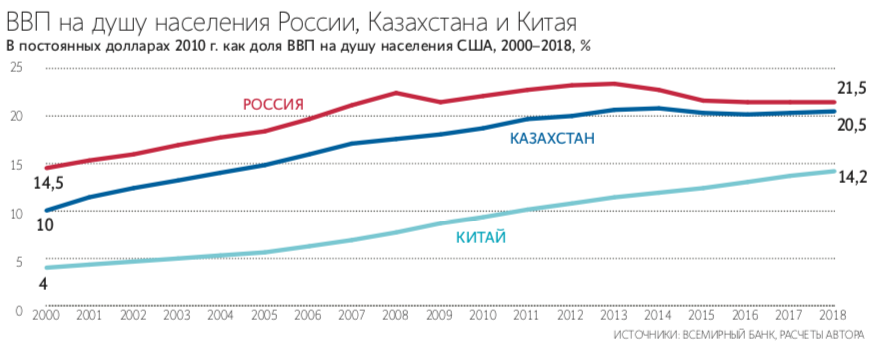
\includegraphics[width=0.68\textwidth]{img/1tbz.png}
    \end{center}
\end{wrapfigure}
\textbf{Авторитарный дедлок.} Более жесткие деспотические режимы политологи называют «авторитарной гегемонией». На выборах здесь авторитарный лидер или правящая партия регулярно получают от 75 до 99\% голосов. Что, однако, свидетельствует не об их популярности, а о том, что они оказывают гораздо более систематическое давление на оппозицию, независимые СМИ и нелояльные элитные группы, т. е. отличаются от предыдущего типа резко возрастающим уровнем репрессивности. Встречаются они сегодня почти исключительно в Азии, Африке и бывшем СССР.

Как показывает опыт ряда азиатских стран, эволюция режима от первого типа ко второму часто происходит на фоне ухудшения экономической динамики. По мере того как экономика играет все меньшую роль в обеспечении легитимности и устойчивости режима, все большую роль начинают играть две другие опоры: репрессии и идеология. В информационной политике режим переходит от фильтрации и ограничения информации к агрессивной пропаганде. Начинаются систематические преследования гражданского активизма, появляются нормы, позволяющие в уголовном порядке преследовать за слова, криминализуется уличная активность граждан.

Именно переход от режима конкурентного авторитаризма к авторитарной гегемонии составил политическое содержание последнего путинского периода – с 2013 по 2019 г. А геополитическая конфронтация выступила в качестве той идеологической рамки, которая легитимирует возрастающую репрессивность.

Хотя Россия выглядит сегодня гораздо более авторитарной страной, чем в 2012 г., этот переход, видимо, следует считать пока незавершенным. Наверное, играют свою роль развитая социальная инфраструктура мегаполисов, уровень европеизированности элит, глубина проникновения интернета и социальных медиа. Ну, и разумеется, экономический застой. Несмотря на это, Путин вряд ли оставит свои усилия по девестернизации России. И это бесплодное (в исторической перспективе) перетягивание каната скорее всего останется главным сюжетом финальной фазы его политической карьеры.


\newpage
\section[Евгений Пригожин]{Пригожин Евгений Викторович}

\textit{Бизнесмен, владелец группы «Конкорд» и ЧВК «Вагнер»}

\textit{Источник \url{https://www.rbc.ru/person/63d280069a79473d6f5e3ce6}}

\textbf{Молодость, образование, родители.} Евгений Пригожин родился в Ленинграде. Его мать Виолетта Кировна Пригожина была медиком и работала в больнице. Отец Виктор Евгеньевич Пригожин рано умер, и ребенка воспитывал отчим Самуил Жаркой. Будучи лыжным инструктором, Жаркой приобщил его к беговым лыжам. В 1977 году Пригожин окончил ленинградскую спортивную школу-интернат № 62 (ныне колледж олимпийского резерва № 1), где учился вместе с пловцом Владимиром Сальниковым и гимнастом Александром Дитятиным, которые впоследствии стали трехкратными чемпионами московской Олимпиады. После школы поступил в Ленинградский химико-фармацевтический институт, получил специальность «провизор-фармацевт». В 2018 году в одном из интервью он сообщал, что институт не закончил.

\textbf{За что сидел Пригожин.} Агентство «Росбалт» (Минюст включил его в реестр СМИ-иноагентов) сообщало, что в ноябре 1979 года Куйбышевский районный народный суд Ленинграда приговорил Пригожина к двум с половиной годам лишения свободы условно по обвинению в краже. По данным Forbes, в 1981 году Ждановский народный районный суд Ленинграда приговорил Пригожина по новым обвинениям в краже, мошенничестве, вовлечении несовершеннолетнего в преступную деятельность и разбое к 13 годам колонии. В 1988 году Пригожин был помилован.

\textbf{Ресторатор, бизнес, карьера.} В 1990 году он стал заниматься бизнесом, начав с продажи хот-догов. Как пишет Forbes, этот бизнес он открыл вместе с отчимом, и часть производства находилась в квартире Пригожина. «Горчицу к хот-догам замешивали прямо у меня на квартире. [...] Приходилось платить бандитам с каждого ларька по \$100», — приводит издание его слова.

В 1991–1997 годах Пригожин управлял сетью частных продовольственных магазинов «Контраст», в 1995 году открыл бар-магазин «Винный клуб» на Васильевском острове в Санкт-Петербурге. В 1996 году, после знакомства с ресторатором Тони Гиром, открыл первый «элитный» ресторан города — «Старая таможня», после появились «Русский китч», «Семь сорок» и «Строгановский дворец».
В том же 1996 году Пригожин основал компанию «Конкорд кейтеринг».

В 1997 году Пригожин открыл ресторан на теплоходе, который получил название New Island и стал на тот момент самым дорогим рестораном Петербурга.
В 1999 году в New Island ужинали премьер-министр Сергей Степашин и директор-распорядитель МВФ Мишель Камдессю.

Пригожин продолжал заниматься розничным фастфудом и с 2002 по 2012 год развивал в Петербурге сеть кафе-блинных под придуманным им названием «Блин! Дональт's». Заведения сети позиционировались как социально значимые, с дешевой едой для местных жителей, блюда в меню получали необычные названия — в частности, там был сэндвич «квадрососисон». Бизнесмен планировал открыть до 20 кафе, однако к 2008 году открылось лишь десять, а с 2009 года компания Пригожина начала закрывать рестораны, последний из которых закончил работать в 2012 году. Сеть фактически послужила основой для создания Пригожиным в дальнейшем формата комбинатов питания. В 2016 году, как писал тогда РБК, Пригожин фактически стал монополистом на рынке школьного питания в Москве.

Строительным бизнесом Пригожин начал заниматься в 2000-х годах в Петербурге. В частности, как писала «Фонтанка», «Конкорд» в районе Лахты построил жилой комплекс «Северный Версаль» из 45 трехэтажных домов в стиле архитектуры Петербурга XVIII—XIX веков.

В 2008 году компания Пригожина ООО «Конкорд менеджмент и консалтинг» (входит в группу «Конкорд») получила участок рядом с парком 300-летия Петербурга для строительства Центра водного туризма. В 2011 году компания обратилась в суд, заявив, что городские власти затягивают выделение участка. В 2012 году суды трех инстанций подтвердили права инвестора. К марту 2016 года компания возвела на участке комплекс «Лахта Плаза» из шести жилых зданий общей площадью 41,9 тыс. кв. м.

В 2010 году компания, принадлежащая жене Пригожина, арендовала в центре Петербурга Дом торгового товарищества «Братья Елисеевы», в котором после реконструкции открылся «Магазин купцов Елисеевых». Летом 2016 года компания добилась права приватизировать здание за 740 млн руб.

Компания Пригожина также сотрудничала с Минобороны: за период c конца 2014 года по середину 2015-го структуры «Конкорда» выиграли тендеры на 10,3 млрд руб. на уборку в казармах и учебных заведениях оборонного ведомства, подсчитывал тогда РБК. Связанная с Пригожиным компания «Мегалайн» получила в 2015 году контракт на 3,3 млрд руб. на строительство военной базы в Валуйках в Белгородской области, она же выиграла на конкурсе контракт на 161,6 млн руб. на строительство военного городка в Омской области. В том же году несколько связанных с Пригожиным компаний выиграли тендеры на жилищно-коммунальное обслуживание военных городков в нескольких областях страны.

\textbf{Фабрика троллей Пригожина.} Имя Пригожина связывают с созданным летом 2013 года Агентством интернет-исследований, которое в прессе называли «фабрикой троллей». В США эту структуру обвиняли во вмешательстве в выборы. Сам Пригожин долгое время это опровергал. В феврале 2023 года бизнесмен заявил, что придумал Агентство интернет-исследований. «Я его создал, я им управлял длительное время. Создано оно было для защиты российского информационного пространства от хамской агрессивной пропаганды антироссийских тезисов со стороны Запада», --- заявил Пригожин.

В 2017 году стало известно о создании структурами Пригожина «фабрики медиа», в которую вошли Федеральное агентство новостей, а также другие связанные с ним издания, в частности «Политика сегодня», «Экономика сегодня» и «Народные новости». Согласно расследованию журнала «РБК», к февралю 2017 года ежемесячная аудитория изданий «фабрики медиа» достигла 36 млн человек, превысив аудиторию агентства «РИА Новости» и «Комсомольской правды». Вскоре эти издания вошли в медиагруппу «Патриот».

В США Пригожина обвинили во вмешательстве в выборы 2016 года и в политический процесс. В феврале 2021 года ФБР назвала Пригожина в числе 13 россиян, которые объявлены в розыск за вмешательство в выборы президента США. Ведомство предложило вознаграждение в размере до \$250 тыс. за сведения, которые помогут заключить бизнесмена под стражу. Пригожин назвал действия бюро «шоу с розыском, как в старые ковбойские времена», и потребовал удалить с сайта ФБР объявление о вознаграждении за информацию о нем.

\textbf{ЧВК Вагнер Евгения Пригожина.} Пригожин — основатель частной военной компании (ЧВК) «Вагнер». Журнал «РБК» писал о полигоне у населенного пункта Молькино в Краснодарском крае, который начал использоваться, предположительно, для подготовки бойцов ЧВК в середине 2015 года. В октябре 2015-го о наборе добровольцев в состав ЧВК и участии ее бойцов в наземных операциях в Сирии, а также в конфликте на территории Луганской и Донецкой народных республик сообщала «Фонтанка». ЧВК получила название «Вагнер» в 2014 году по позывному первого командира подразделения, офицера запаса Дмитрия Уткина.

В США и Евросоюзе заявляли о действиях ЧВК «Вагнер» также в Ливии, ЦАР, Судане, Мозамбике и Мали. Госдепартамент заявлял, что деятельность «Вагнера» в Африке мешает работе миротворцев ООН на континенте.

В июле 2018 года в ЦАР для съемок фильма о деятельности ЧВК направились журналист Орхан Джемаль, оператор Кирилл Радченко и режиссер Александр Расторгуев. По пути к месту съемок их машину атаковали неизвестные вооруженные люди. Журналисты погибли, с места убийства россиян пропали деньги, техника и документы.

США и Евросоюз обвиняли ЧВК «Вагнер» в нарушении прав человека на Ближнем Востоке и в Африке и ввели против компании санкции, которые были ужесточены после начала российской спецоперации на Украине. Санкции были введены в 2016 году и против Пригожина, которого обвинили в связях с ЧВК.

Пригожин долгое время отвергал связь с ЧВК, заявляя, что «крайне удивлен самим фактом существования данной компании и не имеет к ее деятельности никакого отношения». Однако в сентябре 2022 года признался, что именно он является ее создателем. В конце октября 2022-го бизнесмен заявил о создании в Санкт-Петербурге «ЧВК Вагнер Центра», в котором «смогут работать специалисты в области оборонных и информационных технологий с целью повышения обороноспособности России».

\textbf{ЧВК Вагнер на Украине.} Соединения ЧВК активно участвовали в боевых действиях на Украине, в частности под Артемовском (украинское название — Бахмут) и в Соледаре.

Летом 2022 года начали появляться сообщения о посещении Пригожиным тюрем с целью вербовки заключенных в ряды «Вагнера».

\begin{fancyquotes}
    Те, кто не хочет, чтобы воевали ЧВК, заключенные, кто рассуждает на эту тему, кто ничего не хочет делать и в принципе кому эта тема не нравится, детей своих на фронт отправьте. Либо ЧВК и зэки, либо ваши дети — решайте сами

    \begin{flushright}
        Пригожин в сентябре 2022 года\\
        о вербовке заключенных для участия в спецоперации на Украине
    \end{flushright}
\end{fancyquotes}

В ноябре 2022 года телеграм-канал GREY ZONE, который в Совете по правам человека связали с ЧВК «Вагнер», опубликовал видео убийства мужчины, которого назвали бывшим бойцом ЧВК Евгением Нужиным, участвовавшим в спецоперации. На видео мужчина называет свое имя и дает интервью украинским журналистам, заявляя, что добровольно перешел на сторону Киева. Затем Нужина показывают в темном помещении, и его голова примотана к кирпичам скотчем. Мужчина рассказывает, что 11 ноября 2022 года он находился на улице Киева, где получил удар по голове, в результате чего потерял сознание. «Очнулся в этом подвале, где мне сообщили, что меня будут судить», — говорит мужчина на записи, после чего получает удары кувалдой по голове.

После пленения Нужин в интервью украинскому журналисту Юрию Бутусову рассказал, что сам родом из города Перевоз в Нижегородской области и в 1999 году был осужден на 24 года лишения свободы за убийство человека, а затем из-за неудачного побега ему добавили еще четыре года.

Пригожин, комментируя видео, назвал его «прекрасной режиссерской работой». «Что касается окувалдованного, то в данном шоу видно, что он не нашел счастья в Украине, а встретился с недобрыми, но справедливыми людьми», — отметил он.

Позже Пригожин обратился к генпрокурору с просьбой провести доследственную проверку по факту убийства Нужина. 15 ноября уполномоченная по правам человека Татьяна Москалькова заявила РБК, что следственные органы занялись проверкой.

23 ноября Европарламент принял резолюцию, в которой Россия называется страной — спонсором терроризма в связи с военными действиями на Украине. В документе также содержался призыв к странам ЕС признать ЧВК «Вагнер» и входящий в Росгвардию 141-й полк имени Ахмата Кадырова террористическими организациями. После этого пресс-служба Пригожина сообщила, что тот отправил в Европарламент в футляре из-под скрипки «брендированную кувалду [...] с, вероятнее всего, бутафорскими следами крови».

В январе 2023 года США объявили ЧВК «Вагнер» транснациональной преступной организацией. В ответ Пригожин написал письмо в Белый дом с просьбой прояснить, какие преступления совершала эта организация.

Пригожин неоднократно критиковал власти Петербурга и губернатора Александра Беглова. В июле 2022 года он обвинил губернатора в создании помех для бизнеса, после того как структуры, связанные с предпринимателем, не получили контракт на обустройство территории «Горская» и разработку доверили другой компании, несмотря на инвестиционное соглашение. В администрации Петербурга эту точку зрения назвали частным мнением бизнесмена, отстаивающего свои интересы. Беглов заявлял, что действия правительства Петербурга вызывают критику со стороны некоторых «богатых людей, влиятельных людей, которые могут налом проплачивать определенные вещи», не уточняя, кого конкретно имеет в виду. В Кремле, комментируя подобные высказывания Пригожина, заявили, что тот, как предприниматель, «болеет душой за то, что происходит».

\textbf{Призыв к мятежу и уголовное дело.} Вечером 23 июня Пригожин заявил, что российские военные нанесли удар по лагерю ЧВК «Вагнер», в результате чего погибло «погибло огромное количество бойцов». Он обвинил в этом «военное руководство» и пообещал ответ. Позже пресс-служба основателя ЧВК распространила заявление Пригожина, в котором он уточнил, что его намерение «ответить» --- это «не военный переворот, а марш справедливости».

Минобороны утверждения Пригожина опровергло, назвав их «информационной провокацией». В ведомстве подчеркнули, что вооруженные силы «продолжают выполнение боевых задач на линии соприкосновения с вооруженными силами Украины».

Вскоре ФСБ и Генпрокуратура отчитались о возбуждении уголовного дела против Пригожина по статье 279 Уголовного кодекса по факту организации вооруженного мятежа. В ФСБ заявили, что заявления и действия Пригожина фактически являются призывами к началу вооруженного гражданского конфликта на территории и призвали бойцов ЧВК задержать своего лидера. «Призываем бойцов ЧВК не совершать непоправимой ошибки, прекратить любые силовые действия против российского народа, не выполнять преступные и предательские приказы Пригожина, принять меры к его задержанию», — говорилось в заявлении.

Обратился к бойцам ЧВК и генерал Сергей Суровикин. «Я обращаюсь к бойцам и командирам ЧВК «Вагнер». Мы вместе с вами прошли трудный тяжелый путь. Мы вместе с вами воевали, шли на риски, несли потери, вместе побеждали. Мы одной крови. Мы воины... Пока не поздно, нужно и необходимо подчиниться воле и приказу всенародно избранного президента. Остановить колонны, вернуть их в пункты постоянной дислокации», — сказал он в видео, опубликованном военкором Андреем Руденко.

Вечером 24 июня президент Белоруссии Александр Лукашенко сообщил, что провел переговоры с Евгением Пригожиным, они достигли договоренности об остановке движения бойцов ЧВК по территории России. Глава Белоруссии заявил, что бойцам Пригожина дадут гарантии безопасности. Основатель «Вагнера» заявил, что разворачивает свои колонны и уходит в полевые лагеря «согласно плану».

27 июня дело о мятеже было закрыто. Лукашенко заявил, что Пригожин приехал в Белоруссию. «Как я и обещал, если вы хотите какое-то время у нас перекантоваться и прочее, мы вам поможем. Естественно, за их счет», — заявил президент Белоруссии.

Путин заявил, что «организаторы мятежа, предали свою страну и народ». Он также заявил, что содержание ЧВК «Вагнер» полностью обеспечивалось государством. По словам президента, с мая 2022 года по май 2023-го на денежное содержание и стимулирующие выплаты ЧВК государство заплатило 86 млрд и 262 млн руб. «При всем том, что само содержание «Вагнера» было на плечах государства, за год собственник компании «Конкорд» через «Военторг» получил, заработал от государства, поставляя продукты питания и оказывая услуги по питанию в армии, заработал 80 миллиардов рублей», — сказал Путин. Он добавил, что надеется на то, что «в ходе этих работ никто ничего не украл или, скажем так, украл поменьше». По его словам, с этим еще предстоит разобраться.

\textbf{Катастрофа самолета в Тверской области.} Вечером 23 августа 2023 года в Тверской области разбился самолет Embraer Legacy, совершавший рейс Москва — Санкт-Петербург. Как сообщили в МЧС, на борту находились 10 человек, все они погибли. В Росавиации сообщили, что Пригожин был в списке пассажиров самолета. Позже ведомство уточнило, что, по данным авиакомпании, которой принадлежал самолет, бизнесмен действительно был на борту. Также там находится командир ЧВК «Вагнер» Дмитрий Уткин.

Как 24 августа сообщил Владимир Путин, Пригожин в день авиакатастрофы вернулся из Африки. Президент также рассказал, что знал бизнесмена «с начала 90-х годов». «Это был человек сложной судьбы, и ошибки у него были серьезные в жизни, добивался он результатов нужных — и для себя, и для, когда я его просил, для общего дела, как в эти последние месяцы. Он был талантливый человек, талантливый бизнесмен», — добавил Путин.

27 августа СК сообщил, что экспертиза подтвердила гибель Пригожина и остальных пассажиров самолета.

\textbf{Личная жизнь, жена, дети.} Пригожин женат, у него трое детей. Члены семьи Пригожина, в том числе его дети Полина и Павел, в 2022 году попали под санкции ряда западных стран. Под санкции ЕС и Канады также попала мать Виолетта Пригожина (1939 г.р.). Но в марте 2023-го она смогла добиться аннулирования ограничений, введенных против нее Евросоюзом. Суд ЕС установил, что она не владеет компанией «Конкорд Менеджмент и Консалтинг», как считал Брюссель, а родственных связей для включения в санкционный список недостаточно.

В 2003 году Пригожин вместе с детьми Полиной и Павлом написал книгу сказок «Индрагузик», в которой описана сказочная страна Индрагузия.

В сентябре 2022 года Пригожин на странице своей пресс-службы в соцсети «ВКонтакте» сообщил, что его сын в возрасте 18 лет прошел службу в вооруженных силах и через месяц после армии «поехал на войну в Сирию». «С тех пор он постоянно находился и находится в горячих точках в составе ЧВК «Вагнер», где и получил свой первый Черный крест (награда ЧВК. — РБК)», — говорилось в сообщении.

Пригожин награжден орденом «За заслуги перед Отечеством» IV степени «за достигнутые трудовые успехи, значительный вклад в социально-экономическое развитие Российской Федерации, заслуги в освоении космоса, гуманитарной сфере, укреплении законности, активную законотворческую и общественную деятельность, многолетнюю добросовестную работу», и медалями ордена «За заслуги перед Отечеством» I и II степеней. Также в публичных источниках есть фотографии Пригожина со звездами Героя России, Героя Донецкой и Луганской народных республик. В Кремле на вопрос о присвоении Пригожину звания героя закрытым указом президента заявили лишь, что все открытые указы публикуются.

\newpage
\section{Еда на планете становится дефицитом}

\textit{Что будет с ценами на продукты в России и мире}

\textit{Почему продукты на планете постоянно дорожают}

\textit{Источник \url{https://www.kp.ru/daily/27547.5/4814137/}}

Продовольственный кризис \ex{разворачивается}{is unfolding} на нашей планете прямо сейчас. Трудно в это поверить, глядя на переполненные полки супермаркетов. Но нехватку еды, по данным ООН, ощущают на себе уже около 2 млрд человек в 80 странах. А около 20 тысяч человек ежедневно умирает от голода и его последствий.

Последний резкий рост цен на продовольствие случился в 2020 - 2022 годах. И это был уже третий \ex{скачок}{jump} за последние 15 лет. В первой половине 2023 года цены вроде пошли вниз, но в июле --- новый рост. Так в чем причины нехватки еды на планете?

\textbf{Причина № 1. Конфликты и войны.} Это одна из главных причин: 70\% голодающих живут на территориях, где происходят боевые столкновения. И \ed{нынешнее}{нынешний}{present, current} вооруженное \ex{противостояние}{confrontation} на Украине тоже ударило по самым чувствительным точкам --- поставкам энергоносителей, удобрений и сельхозпродукции.

До начала боевых действий Россия и Украина экспортировали на мировые рынки значительные доли пшеницы (18\% и 10\%), ячменя (14\% и 12\%), \ed{подсолнечного масла}{подсолнечное масло}{sunflower oil} (26\% и 37\%). После начала кризиса объемы экспорта сельхозпродукции с Украины сократились на 30 - 40\%. Странам Европы, Азии и Африки пришлось искать новых \ed{поставщиков}{поставщик}{supplier} и выстраивать новые пути доставки, что привело к росту цен.

\textbf{Причина № 2. Природные катаклизмы.} Особенно от этого страдают жители Африки и Юго-Восточной Азии. В 2021 - 2022 годах дефицит осадков здесь достигал 80\%. Грустный итог: с середины 2021 года по апрель 2022-го в Кении и Эфиопии погибло около 3 млн голов скота. Похожая ситуация в Сомали.

А в западной части континента все наоборот: наводнения уничтожают пахотные земли. По оценке ООН, производительность сельского хозяйства в Африке по итогам 2022 года снизилась на 34\%.

Страдают от аномалий погоды Индия, Китай, Южная Америка. Постоянно дают о себе знать течения Эль-Ниньо и Ла-Нинья: температура воды в экваториальной части Тихого океана меняется, влияя на осадки в Азии и Южной Америке.

Не жалеет погода и США. Из-за жары 2022 года урожай пшеницы в Америке сократился вдвое, а на юге Европы погодные аномалии принесли убытки на миллиарды евро...

\textbf{Причина № 3. Энергетический кризис.} Для производства, доставки, упаковки, хранения продуктов нужна энергия --- газ, нефть, электричество. А газ и нефть резко дорожали в 2021 - 2022 годах (цена на голубое топливо взлетала в несколько раз). Последствия этого скачка мир ощущает до сих пор.

\textbf{Причина № 4. Нехватка удобрений.} Современное сельское хозяйство \ex{немыслимо}{unthinkable} без минеральных удобрений, а они постоянно дорожают. С 2022 года этот рынок залихорадило снова: сказались \ed{перебои}{перебой}{interruption} с поставками из России, введение экспортных квот Китаем и подорожавший в 2022 году природный газ --- ключевой компонент при изготовлении азотных удобрений. Проблемы с газом заставили многие страны сократить собственное производство.

Итог --- цены на отдельные виды удобрений подскочили в три раза, что сразу ударило по стоимости продуктов. Нехватка удобрений наверняка скажется и на урожайности.

На мировые цены влияет множество факторов. Стоимость отдельных продуктов может не только расти --- бывает, что цены снижаются. Но, как шутят эксперты, если цены падают на биржах, они не падают на наших кухонных столах. Ведь стоимость сельхозтоваров формируется главным образом после того, как они покидают фермы. Речь о затратах на энергию, обработку, упаковку, доставку, рабочую силу... И каждая из этих позиций из года в год прибавляет в цене. В итоге по пути в магазин продукты дорожают в 2 - 3 раза, а то и больше.

В этом году быстрее других продуктов дорожают зерно, рис, какао и апельсины. Давайте выясним, почему.

\textbf{Нерациональное зерно.} Мировой рынок зерновых \ex{трясет}{is shaking}. В начале марта цены на пшеницу достигали исторического максимума --- \$12,09 за бушель (единица объема для измерения зерна, один бушель равен в среднем 27,21 кг). Затем они падали, снова росли, особенно после того, как Россия вышла из «зерновой сделки». Напряжение между Россией и Украиной играет здесь важную роль, поскольку обе страны --- крупные поставщики этого продукта на мировой рынок.

Сейчас стоимость пшеницы на биржах упала до 6,5 доллара за бушель, но как цены поведут себя дальше, сказать трудно. С одной стороны, замедляется спрос на зерновые корма. С другой - к увеличению потребления зерновых ведет рост населения планеты.

Мировая торговля зерном к 2031 году должна вырасти на 15\%, а пшеница в общем объеме занимает около 40\%. И Россия останется одним из лидеров по экспорту пшеницы на мировой рынок (доля - более 20\%). Оптимизма добавляют и хорошие урожаи в нашей стране.

Сообщения о том, что в России из-за ситуации на зерновом рынке может подорожать хлеб, на днях опроверг Минсельхоз. Здесь уверили: обеспеченность России зерном намного превышает внутренние потребности. Поэтому рост цен на хлеб в этом году будет не выше общей инфляции (по плану --- не более 6,5\%).

\textbf{Рис --- благородное дело.} Цены на рис в этом августе достигли многолетних максимумов. Например, эталонный для экспортеров в Азии тайский белый рис стоил \$650 за тонну - это на 50\% больше, чем в августе прошлого года. Особенно быстро цена на рис стала расти с июля, после объявления Всемирной метеорологической организацией ООН о появлении Эль-Ниньо, вызывающего засухи.

Кроме того, недавно Индия --- крупнейший поставщик риса --- заявила о запрете экспорта 80\% этой продукции, чтобы сдержать рост внутренних цен на этот стратегический для страны товар. Временно запретили экспорт риса ОАЭ и Россия. Но стратегическим продуктом рис остается не только для Индии, а для 40\% населения Земли, особенно в Азии. Он обеспечивает базовое питание 3 млрд человек. И экономисты \ex{опасались}{they feared}, что осенью цены на рис могут вырасти вдвое к прошлому году.

России рост цен пока не грозит. Во-первых, наша страна сама выращивает рис. Его мы ежегодно производим больше миллиона тонн, и этого хватит, чтобы удовлетворить внутренний спрос. Во-вторых, правительство вовремя ввело ограничения на вывоз этого продукта из страны --- теперь у аграриев нет \ed{искушения}{искушение}{temptation} экспортировать рис, пользуясь выгодными для себя ценами.

\textbf{Чао, какао!} Какао-бобы, а точнее, какао-масло, которое из них производят, --- один из главных ингредиентов в производстве шоколада. Дефицит и подорожание какао приведет к росту цен на всю кондитерку.

Стоимость какао-масла выросла с начала года уже на 20\% и приблизилась к максимальному уровню за последние полвека, преодолев в июле \ed{отметку}{отметка}{mark} 3500 долларов за тонну. Причина --- плохая погода в Западной Африке. Ведь как раз на две страны этого региона --- Кот-д' Ивуар и Гану --- приходится 60\% мирового производства какао.

Основатель фабрики ShokoBox Андрей Шарков уверен, что повышения цен на шоколад не избежать и России. Причины -- \ex{подорожание}{rise in price, price hike} сырья на мировых рынках и ослабление рубля. Ведь наш шоколад производится из импортных компонентов.

\begin{fancyquotes}
    Думаю, что осенью нам следует ожидать роста цен на шоколадные изделия в среднем на 10\%, - рассказал Андрей Шарков «КП». - При этом их качество станет хуже.
\end{fancyquotes}

Многие производители попытаются компенсировать рост цен заменой натурального какао-масла дешевыми заменителями. Российский рынок не слишком требователен к качеству, но те, кто ценит настоящий шоколад, почувствуют разницу. И качественные продукты без заменителей подорожают еще больше. Мой прогноз --- на 20\%.

\textbf{Нету сладких апельсинов.} Бразилия была и остается крупнейшим мировым поставщик\'{о}м концентрата для производства апельсинового сока. Но в этом году в стране \ex{неурожай}{bad harvest, crop failure}, цены поползли вверх. Масла в огонь подлили неблагоприятная погода и плохой урожай цитрусовых в США, Мексике и Испании. В итоге за год стоимость фунта замороженного концентрата апельсинового сока выросла с 2 до 3 долларов.

В России цены на апельсины росли с 2020 года. А этим летом наши торговые сети столкнулись с их дефицитом, так что дорожать они, видимо, будут и дальше. Замороженный концентрат апельсинового сока уже подорожал в России на 30\%. Что неизбежно приведет к пропорциональному росту цен.

\textbf{В ТЕМУ}

\textbf{Пицца против окрошки}

\textbf{Национальные блюда тоже бьют по кошельку}

Официальные цифры инфляции не всегда отражают то, как ощущают на себе подорожание продуктов обычные граждане. В ЕС, например, продовольственная инфляция составляет порядка 12,5\%. Но если взять популярную в Италии пиццу «Маргарита», то ее цена в январе 2023-го, по данным Bloomberg, выросла к январю 2022 года на 25\%. Притом, что официальная инфляция в Италии за этот период составила 10,7\%. А все потому, что сильно взлетели цены на сыр и муку.

Похожая ситуация с национальным блюдом испанцев паэльей. Она за год подорожала на 19\% при общей инфляции в Испании 6\%. Сказался рост цен на оливковое масло, овощи и бобы.

На 20\% подорожал классический британский завтрак (сюда входят бекон, колбаски, яйца, тосты и напиток). Причина - рост цен на молоко, хлеб и яйца. Кстати, в США именно яйца рекордно взлетели в цене - в начале 2023 года они стоили на 60\% дороже, чем годом ранее.

А вот окрошка подорожала за год всего на 6\%. Виноваты в основном овощи. Редис подорожал к прошлому году почти на треть, огурцы - на 25\%, зеленый лук - на 5\%. Даже квас прибавил в цене 6\%. Зато картофель и яйца подешевели.

\textbf{ТОЛЬКО ЦИФРЫ}

29,3\% всего населения планеты испытывают умеренную или серьезную нехватку продовольствия.

Более 345 млн человек столкнутся в 2023 году с «высоким уровнем отсутствия продовольственной безопасности». По сути --- будут \ed{недоедать}{недоедать/недоесть}{to be undernourished, to not eat enough}.

14 из 15 стран с наибольшим отсутствием продовольственной безопасности находятся в Африке.

По данным ФАО ООН и Всемирной продовольственной программы ООН.











